\section{Introduction}

% Genetic data carries information about past evolutionary events
Processes like mutation, recombination, assortative mating and selection leave footprints on genetic variation.
A major goal of population genetics has been to invert this relationship and infer past, unobserved evolutionary events from genetic variation data \citep{schraiber_methods_2015}.
However, with the dramatic increase in our ability to generate whole-genome data,
there is a need for more efficient inference methods that can scale well to over tens of thousands of individuals.

% How has inference been done traditionally?
% Thinking about how processes impact trees, then translating that into summary statistics that can be computed from genetic data.
Although our interest is to infer evolutionary processes from population genetic data,
it is usually simpler to first think about the effects of these processes on the shape of underlying genealogies \citep{wakely_coalescent_2016},
and how this ultimately translates to observed genetic variation.
In the absence of recombination,
a genealogy is a tree that describes the shared ancestry of a sample of DNA molecules (e.g. haploid individuals),
until they ``coalesce'' into a single common ancestor.
The shared ancestry of individuals reflects historical processes that acted upon their ancestors. 
For example, recent contractions in population sizes will lead to genealogies where individuals coalesce relatively recently.

% Describe the ARG
For recombinant DNA,
the genealogy is not a tree but instead a graph that encodes the transmission of genetic material from ancestors to present-day individuals at every point in the genome,
known as the ``ancestral recombination graph'' (ARG).
The ARG records two types of historical events:
coalescences (where separate lineages merge into a common ancestor),
and recombinations (where a single lineage splits into multiple lineages, moving backward in time).
Crucially, ancestors are ``local'' in the sense that only a subset of the ancestors in the entire ARG are associated with each location in the genome.
Thus, one factorization of ARG is into a sequence of correlated marginal trees,
where changes in tree structure are caused by recombination events \citep{kelleher_efficient_2016, kelleher_inferring_2019}.
The branches of these trees have two dimensions:
the time separating descendant from ancestor,
and the length of sequence spanned by the tree containing the branch.
A second factorization is into the minimal set of ancestral haplotypes and transmission paths between these ancestors,
which is equivalent to collapsing coalescence nodes and branches across marginal trees. 

% Describe how mutational density == edge area ==> summary statistics
If a genetic variant is segregating in a sample of present-day individuals, 
then the mutational events leading to that variant can be mapped to particular edges in the ARG. 
In particular, neutral mutations occur on a given edge at a rate proportional to its area.
Thus, the distribution of variant frequency reflects the shape of the underlying ARG. 
More generally, summary statistics of frequencies of neutral variants are noisy measurements of
equivalent summary statistics of branch areas across marginal trees in the underlying ARG \citep{ralph_efficiently_2020}.

A typical strategy for evolutionary inference is to compare summary statistics (based on genotype matrices) to their expectations under a parametrized model.
For example, the site frequency spectrum (SFS) describes the distribution of allele frequencies across sites in the genome,
and is frequently used to infer the demographic histories of natural populations \citep{gutenkunst_inferring_2009, schraiber_methods_2015}.
However, individual statistics that summarize genetic variation cannot capture all aspects of the data that are informative of the underlying processes.
These limitations may be circumvented to some degree by using multiple summary statistics either in a composite likelihood framework or with likelihood-free methods \citep{nielsen_genomic_2005, degiorgio_sweepfinder2_2016, sheehan_deep_2016, caldas_inference_2022, pavlidis_sweed_2013};
and by stratifying data into windows across chromosomes \citep{schrider_shic_2016, flagel_unreasonable_2019, sheehan_deep_2016}.
However, there is inevitably a tradeoff between granularity and informativeness,
both in the choice of summary (from raw genotypes to compact summaries like the SFS) and scope (from single bases to large windows).

% TODO: everything below here is an outline; needs rewording
Assume the underlying ARG for a dataset could be observed. 
Using the ARG as an input would solve many of the issues above \citep{rasmussen_genome-wide_2014}. 
This is because it is simultaneously: 
(A) sufficient, in the sense that it contains all information obtainable from observed genetic data; 
(B) compact, in the sense that shared genetic variation is naturally encoded in marginal trees; 
(C) multiscale, in the sense that the span of ancestral haplotypes and edges naturally reflects the "spatial" and temporal scales at which shared ancestry impacts variation, without arbitrary discretization into windows.

% talk about tree sequence / ARG inference
This core idea of using ARGs for evolutionary inference has two challenges in practice. 
First, we cannot observe the ARG directly but instead we have to infer it. 
There are approaches for inferring ARGs in a more-or-less scalable way \citep{speidel_inferring_2021, kelleher_inferring_2019, zhang_biobank-scale_2023}. 
But these will inevitably contain error (\eg in genotyping, phasing, etc.),
so any inference method using inferred ARGs as input must be able to model error either explicitly or implicitly.
Second, we need some way to ``parameterize'' the ARG in terms of quantities we are interested in. 
This would traditionally be done by specifying some generative process, like the coalescent with recombination,
and calculating likelihood of observed genetic data conditional on this process \citep{fan_likelihood-based_2023}. 
However, these likelihoods are only tractable under a very small class of models. 
Likelihood free inference seems to be the most promising solution,
specially now given recent advances in population genetic simulation tools that allow ARG recording \citep{haller_tree-sequence_2019, kelleher_efficient_2016, ralph_efficiently_2020}. 
%Still, it remains an open problem how to compute a measure of goodness of fit between simulated and inferred ARGs.

Graph neural networks (GNNs), an emerging class of deep learning algorithms, provide a natural way to exploit ARGs for evolutionary inference.
These networks fall into the broader message passing paradigm whereby information is aggregated in neighborhood of nodes,
ultimately yielding an embedding for nodes in a graph \citep{bronstein_geometric_2017, battaglia_relational_2018, hamilton_inductive_2018}..
These node embeddings can then be used for downstream tasks such as node classification, graph classification, and edge prediction.
GNNs can leverage information from genealogies (\ie historical relationships between nodes and the timing of coalescent events) \citep{korfmann_simultaneous_2023},
but they would not take into account additional structure in ARGs induced by the spatial (along the chromosome) and temporal (from parent to child) ordering of nodes.

Here, we present a new method that uses whole-genome genealogies for evolutionary inference.
Our main goal is to develop an architecture that can efficiently use genealogies for inference at different levels.
As a proof-of-concept, we test our method on dating mutations in an ARG.
Our approach, tsNN, outperforms an out-of-the-box graph neural network and current likelihood-based approaches.
Taken together, our results demonstrate that tsNN is a powerful and flexible framework for leveraging information from whole-genome genealogies for evolutionary inference.

\section{Methods} \label{sec:methods}

\subsection{tsNN}
Taking inspiration from the graph neural network literature \citep{rossi_temporal_2020},
we developed an encoder that can take whole-genome genealogies as input and generates node embeddings \plcref{fig:nn}.
In summary, we obtain a lower dimension representation of these genealogies by passing messages between nodes.
We start with an initialized embedding for nodes, and
then we use an update scheme that takes an edge and updates the embedding of both child and parent nodes.
Because the flow of information is structured from parent to child and from left-to-right,
we hoped this neural network would learn a better representation of a tree sequence than a more naive approach,
such as a simpler graph neural network.
The node embeddings can then be decoded to obtain edge (and mutation) embeddings or a tree sequence level embedding.

\begin{figure}[htp]
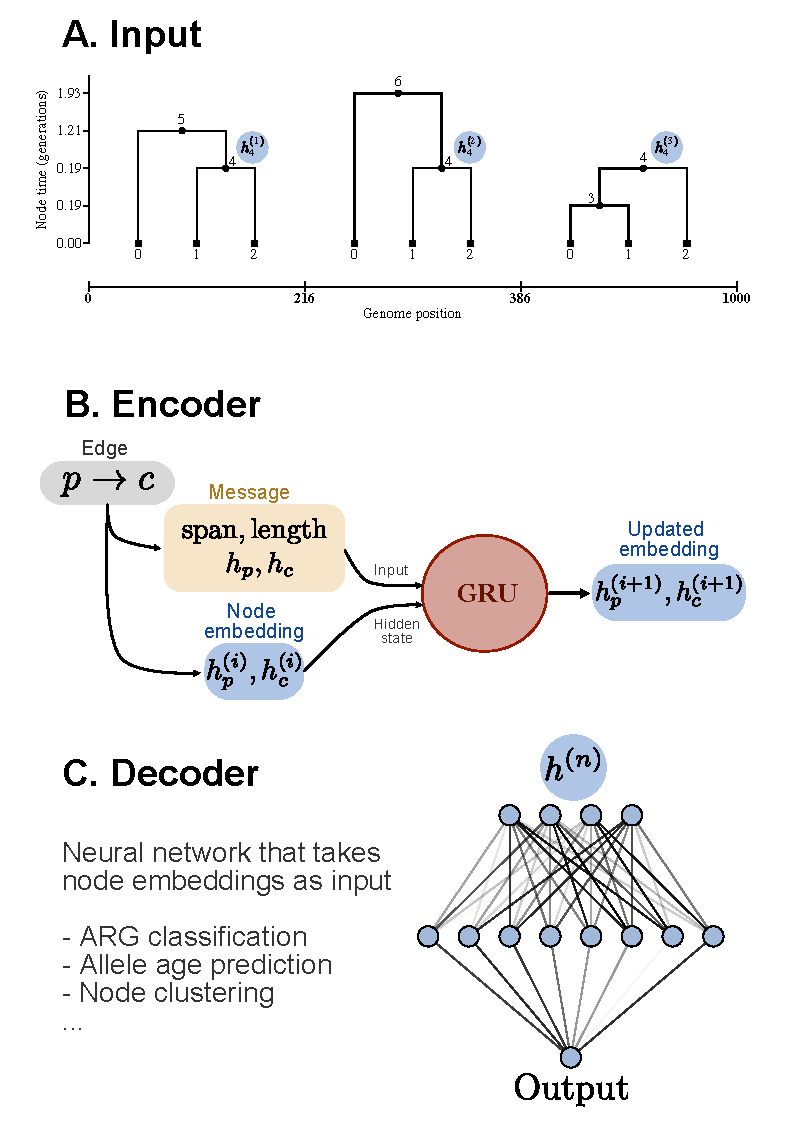
\includegraphics[width=0.8\linewidth]{{tsnn_figs/nn.pdf}}
\centering
\caption[Schematic representation of the tsNN algorithm]{
Schematic representation of the tsNN algorithm.
A) An example tree sequence that can be used as input to tsNN.
Edges that differ from the previous tree are highlighted with thicker lines.
Note how the embedding of node $4$ ($h_4$) is updated with edge differences along the tree sequence.
B) The tsNN encoder updates node embeddings as it iterates over edge insertions along the tree sequence.
The update is done with a Gated Recurrent Unit (GRU) that takes the span and length of the edge along with the node embedding for the parent and child nodes.
C) The node embeddings can be decoded in different ways for a supervised task.
}
\label{fig:nn}
\end{figure}

First, we define an encoder module for obtaining node embeddings.
We randomly (or arbitrarily) initialize a vector with node features $H$ of dimension number of nodes by number of node features.
From a given tree sequence, we also compute a vector $E$ of edge features of dimension number of edges by number of edge features.
We define two edge features: the span (width in number of base pairs that an edge spans, scaled by the mutation rate) and edge length (the number of mutations on an edge).
We traverse the tree sequence over edge differences (from letft-to-right, and optionally from right-to-left), and
with each edge addition, we build a message that is used to update the node features $H$.
The message for the edge that links the parent node $p$ to the child node $c$ is 

$$ m_{pc} = e_{pc} \mathbin\Vert (h_p \mathbin\Vert h_c)$$

where $e_{pc}$ is the row of $E$ for the edge $p-c$, and $h_p$ and $h_c$ are the rows of $H$ for nodes $p$ and $c$.
$h_p$ and $h_c$ are then updated with a Gated Recurrent Unit cell, such that

$$ h^{\mathrm{out}}_p \mathbin\Vert h^{\mathrm{out}}_c = \mathrm{GRU}(m_{pc}, h_p \mathbin\Vert h_c)$$

The node embedding module above can be combined with different neural network architectures to decode the node embeddings to infer parameters at different levels.
For our mutation time task, we first compute edge embeddings,
where for each edge we concatenate the corresponding parent and child node embeddings.
For each mutation, we assign its embedding as the corresponding edge embedding (we ignore mutations that map to more than one edge).
Then, we feed these embeddings into a Multi-layer Perceptron (MLP) of an arbitrary shape with an output size of 1 (one predicted mutation time for each mutation).

\subsection{GNN}

We also tested a simple graph neural network architecture (GNN), similar to \citet{korfmann_simultaneous_2023}.
The GNN leverages topological information, as well as edge features similarly to tsNN.
The GNN performs graph convolutions (passing information between related nodes) to obtain a node embedding.
However, most spatial (along chromosome) information is lost.
These node embeddings can then be decoded in the same way as described above for tsNN.

\subsection{Training and validation simulations}

We used stdpopsim to simulate the ARG of a sample (100 diploid individuals) under the three population Out-of-Africa demographic model (OutOfAfrica\_3G09),
with constant recombination rate of $1.3 \times 10^{-8}$ and mutation rate of $2 \times 10^{-8}$.
To avoid leaking of information from the true simulated ARGs,
we reordered the nodes by mean number of descendants (as opposed to true node times) with the constraint that parent nodes are older the respective child nodes.
The only features, beyond the topologies, that the neural networks saw were edge features (span and length).
Span was scaled by the mutation rate and edge length was computed as the number of mutations on an edge.

We simulated 900 replicate ARGs under this model for training and 100 for validation (note no hyper-parameter tuning was performed).
To compare tsNN and GNN, we simulated 10Kb genomes.
However, we also trained tsNN on 1Mb genomes to understand the relationship between sequence length and accuracy.
We trained both models with mean squared error loss on the $\log_{10}$ transformed mutation times.

\section{Results}

We devised a test to better understand whether a neural network can extract relevant evolutionary information from ARGs.
The process of ARG inference is usually split into two steps:
(i) local tree topology estimation, and 
(ii) inference of branch lengths and node times is performed using a ``molecular clock'' (after mapping mutations onto trees).
The second step is straightforward, but strong coalescent priors are used and dating is heavily affected by issues in the data.
Thus, we reasoned that estimating times from tree sequences is a simple, yet fundamental task in ARG inference.
The choice of estimating mutation times, as opposed to node times, is due to the fact that true nodes are never known in practice,
as the only actual data we can observe are mutations.
Importantly, we sought to estimate mutation times by presenting the neural networks with a modified true ARG,
in which nodes are reordered based on the mean number of descendants.
Further, the network only sees span (scaled by the mutation rate) and edge lengths (as the number of mutations in an edge).

\subsection{Comparing tsNN and GNN}
The fundamental difference between tsNN and GNN is the fact that tsNN induces a particular ordering to updating node embeddings, 
that we hypothesize is important for extracting evolutionary information.
The node embeddings are updated with the edge insertion oder along a tree sequence \plcref{fig:edge_order}.
Because younger haplotypes persist far longer than old haplotypes, 
a young haplotypes will be involved in many more updates than an old one.

\begin{figure}[htp]
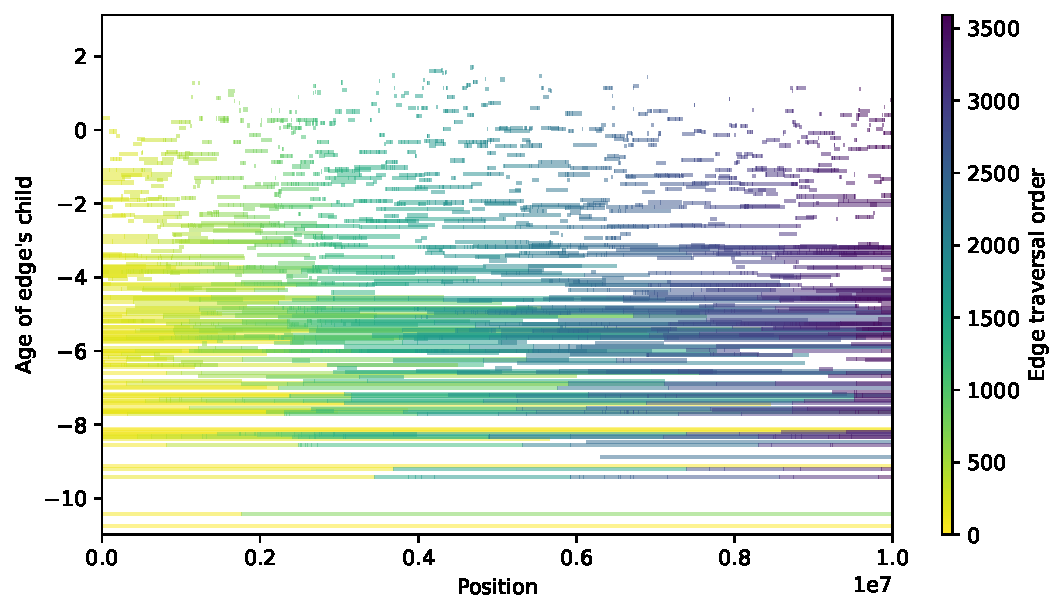
\includegraphics[width=0.9\linewidth]{{tsnn_figs/tseq_edge_diffs.pdf}}
\centering
\caption[Edge traversal order in tsNN]{
Edges in an arbitrary tree sequence, with the edge traversal order in tsNN represented by a color gradient.
Edges are represented as horizontal lines, where the y-axis denotes the age of an edge's child and x-axis denotes the left and right positions along the chromosome.
}
\label{fig:edge_order}
\end{figure}

We found that tsNN outperforms the GNN in inferring mutation times \plcref{fig:tsnn_vs_gnn},
even though the GNN architecture has about 6 times more parameters (560,000 trainable parameters in the GNN versus 90,000 parameters in the tsNN).
Current dating algorithms can achieve an $R^2$ of around $0.9$ \citep{wohns_unified_2022} using the true ARG.
Our model trained on 10Kb sequences fail to properly estimate the time of mutations younger than $\log_{10}^2$ generations,
greatly affecting overall accuracy.

\begin{figure}[htp]
\centering
\begin{subfigure}[b]{.51\linewidth}
    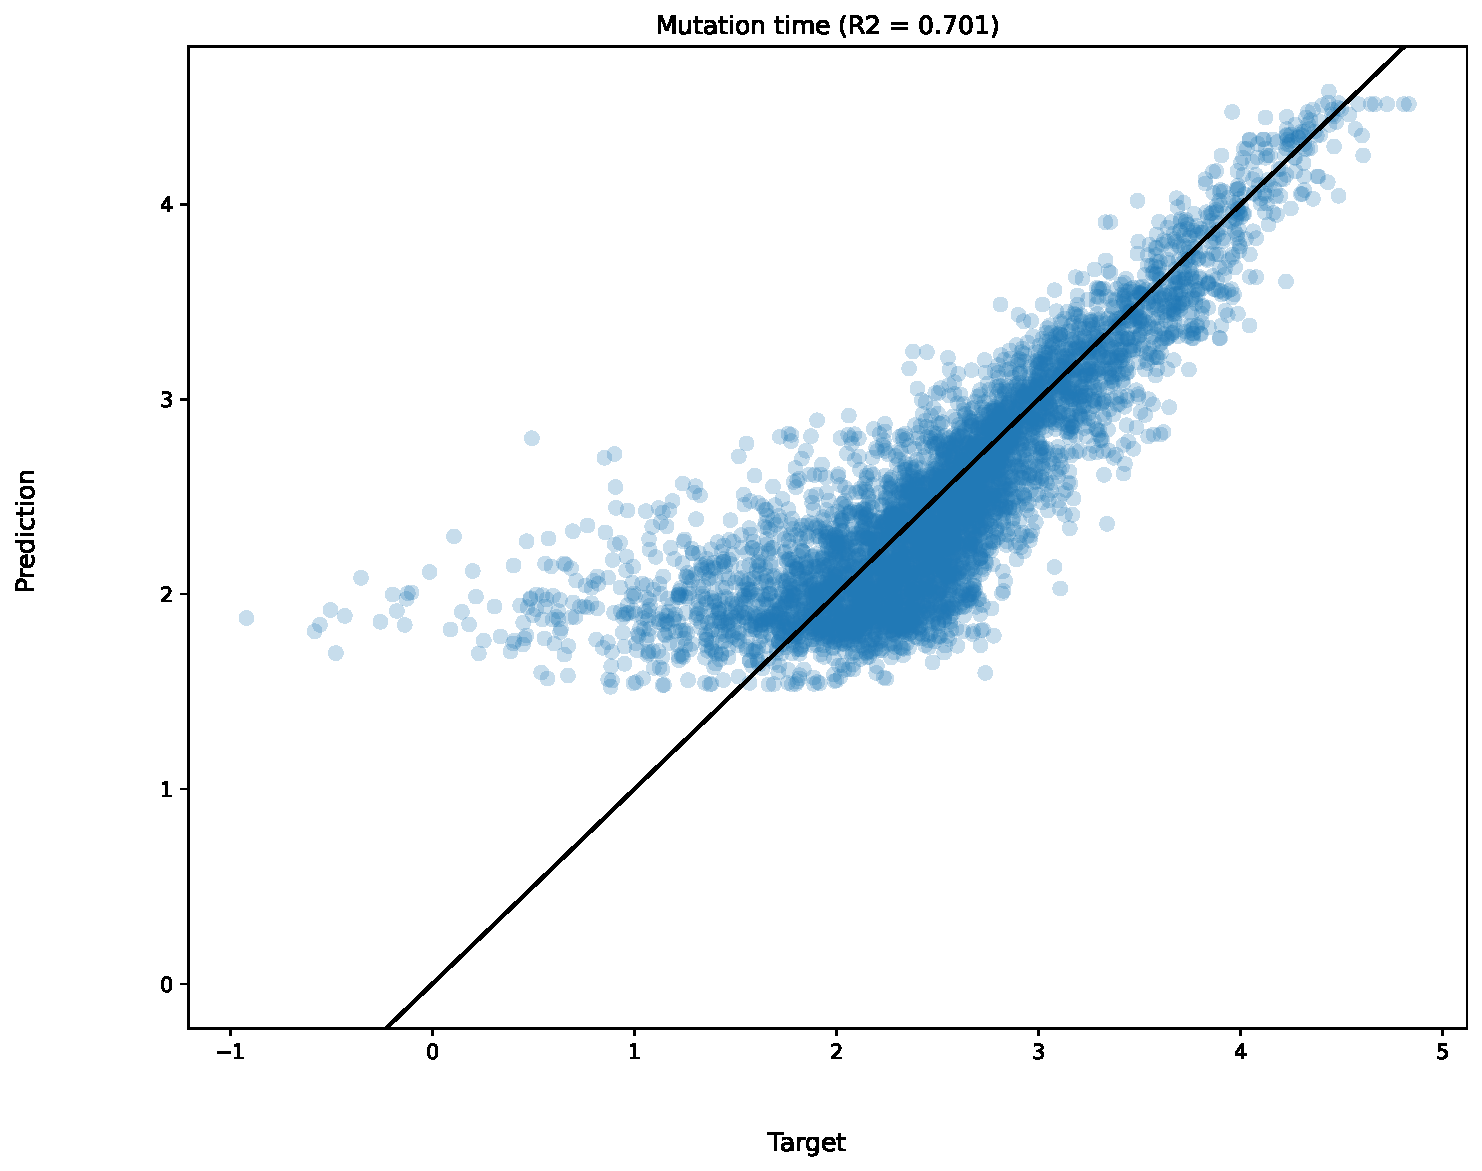
\includegraphics[width=\linewidth]{tsnn_figs/tsnn_ntrain_900_clen_10kb_mut-rate_2e-8_ssize_100_scatter_val_redone.pdf}
\caption{tsNN}\label{fig:10kb_tsnn}
\end{subfigure}
\hfill
\begin{subfigure}[b]{.51\linewidth}
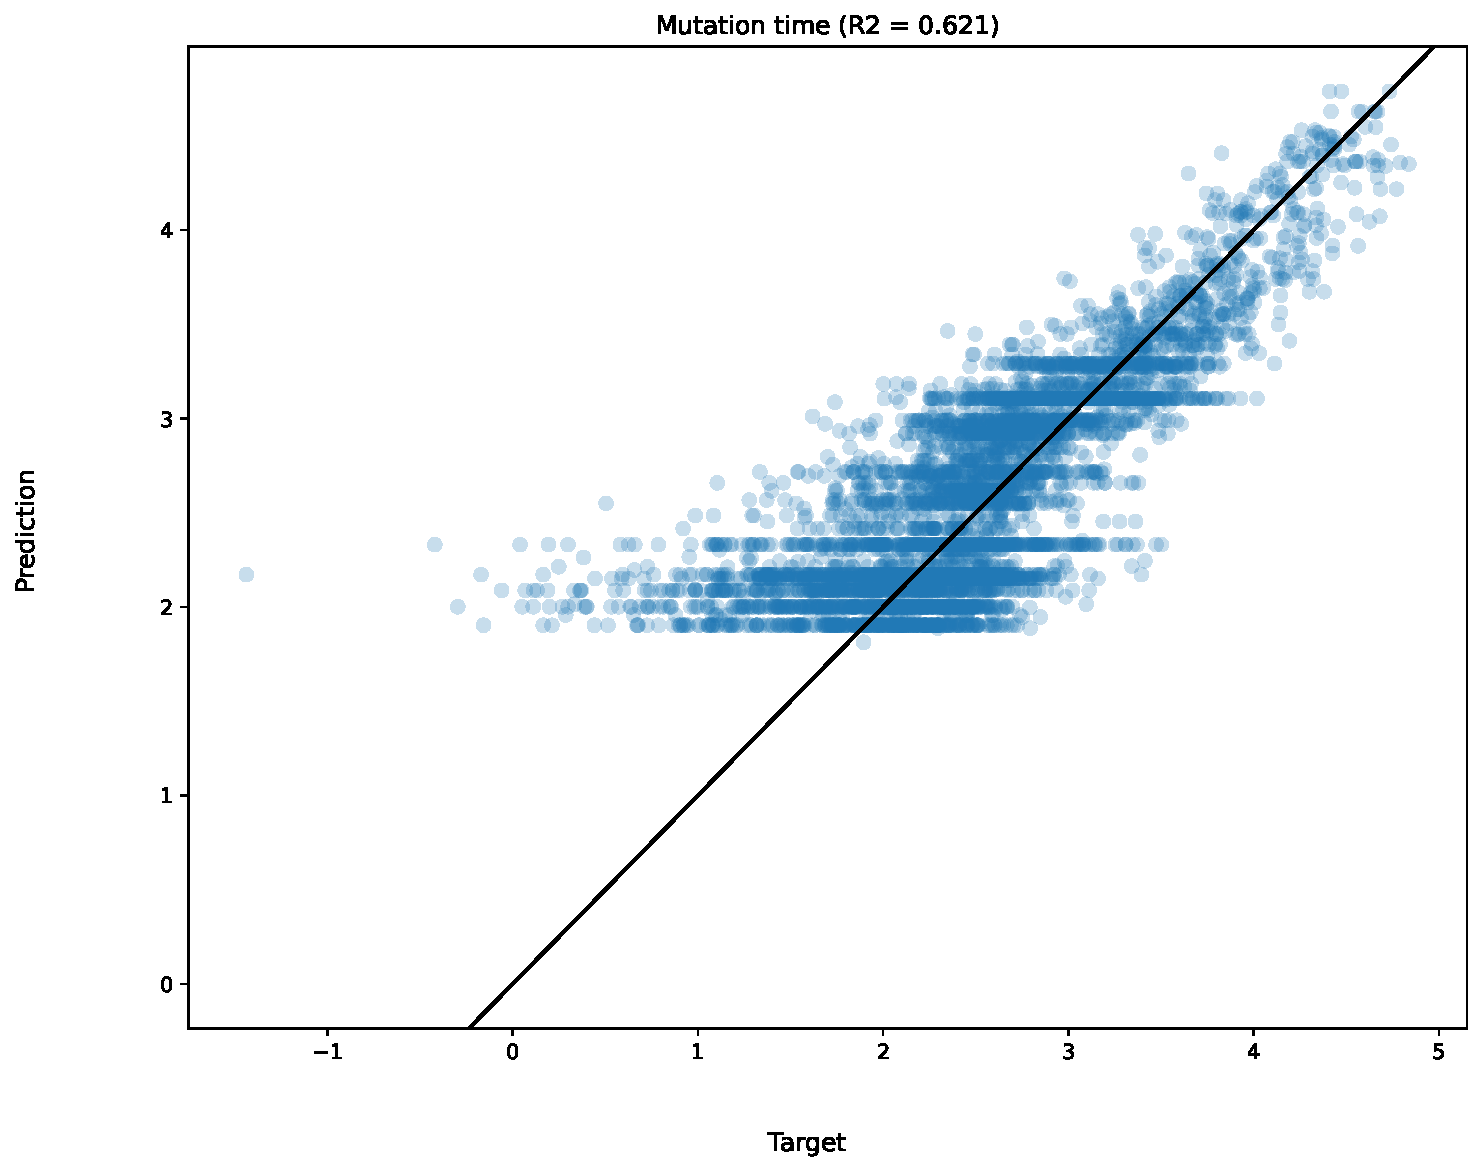
\includegraphics[width=\linewidth]{tsnn_figs/gnn_ntrain_900_clen_10kb_mut-rate_2e-8_ssize_100_nnodefeat_16_scatter_val.pdf}
\caption{GNN}\label{fig:10kb_gnn}
\end{subfigure}
\caption[Accuracy of tsNN and GNN in predicting mutation times]{
Accuracy of tsNN and GNN in predicting mutation times.
Scatterplots show predicted against target mutation times for 100 tree sequences.
Times are $\log_{10}$ transformed.
}
\label{fig:tsnn_vs_gnn}
\end{figure}

\subsection{Improving inference of mutation times}

The failure to correctly infer the ages of young mutations could be caused by two factors: 
(i) the training dataset does not contain enough young mutations, and
(ii) the model needs larger sequences (more than 10Kb) to better learn the recombination clock (\ie the spans of young haplotypes will not be artificially truncated by 10Kb).
To test what could be causing this issue,
we changed the training data either by scaling the mutation rate or by increasing the simulated chromosome.
We found that accuracy increases as mutation rates increases \plcref{fig:10kb_7,fig:10kb_6},
suggesting that the number of young mutations does limit learning.
However, increasing the chromosome length increases accuracy even more \plcref{fig:1mb_8}.
Thus, it seems the network is learning the recombination clock and using it to improve prediction of mutation times.

\begin{figure}[htp]
\centering
\begin{subfigure}[b]{.51\linewidth}
    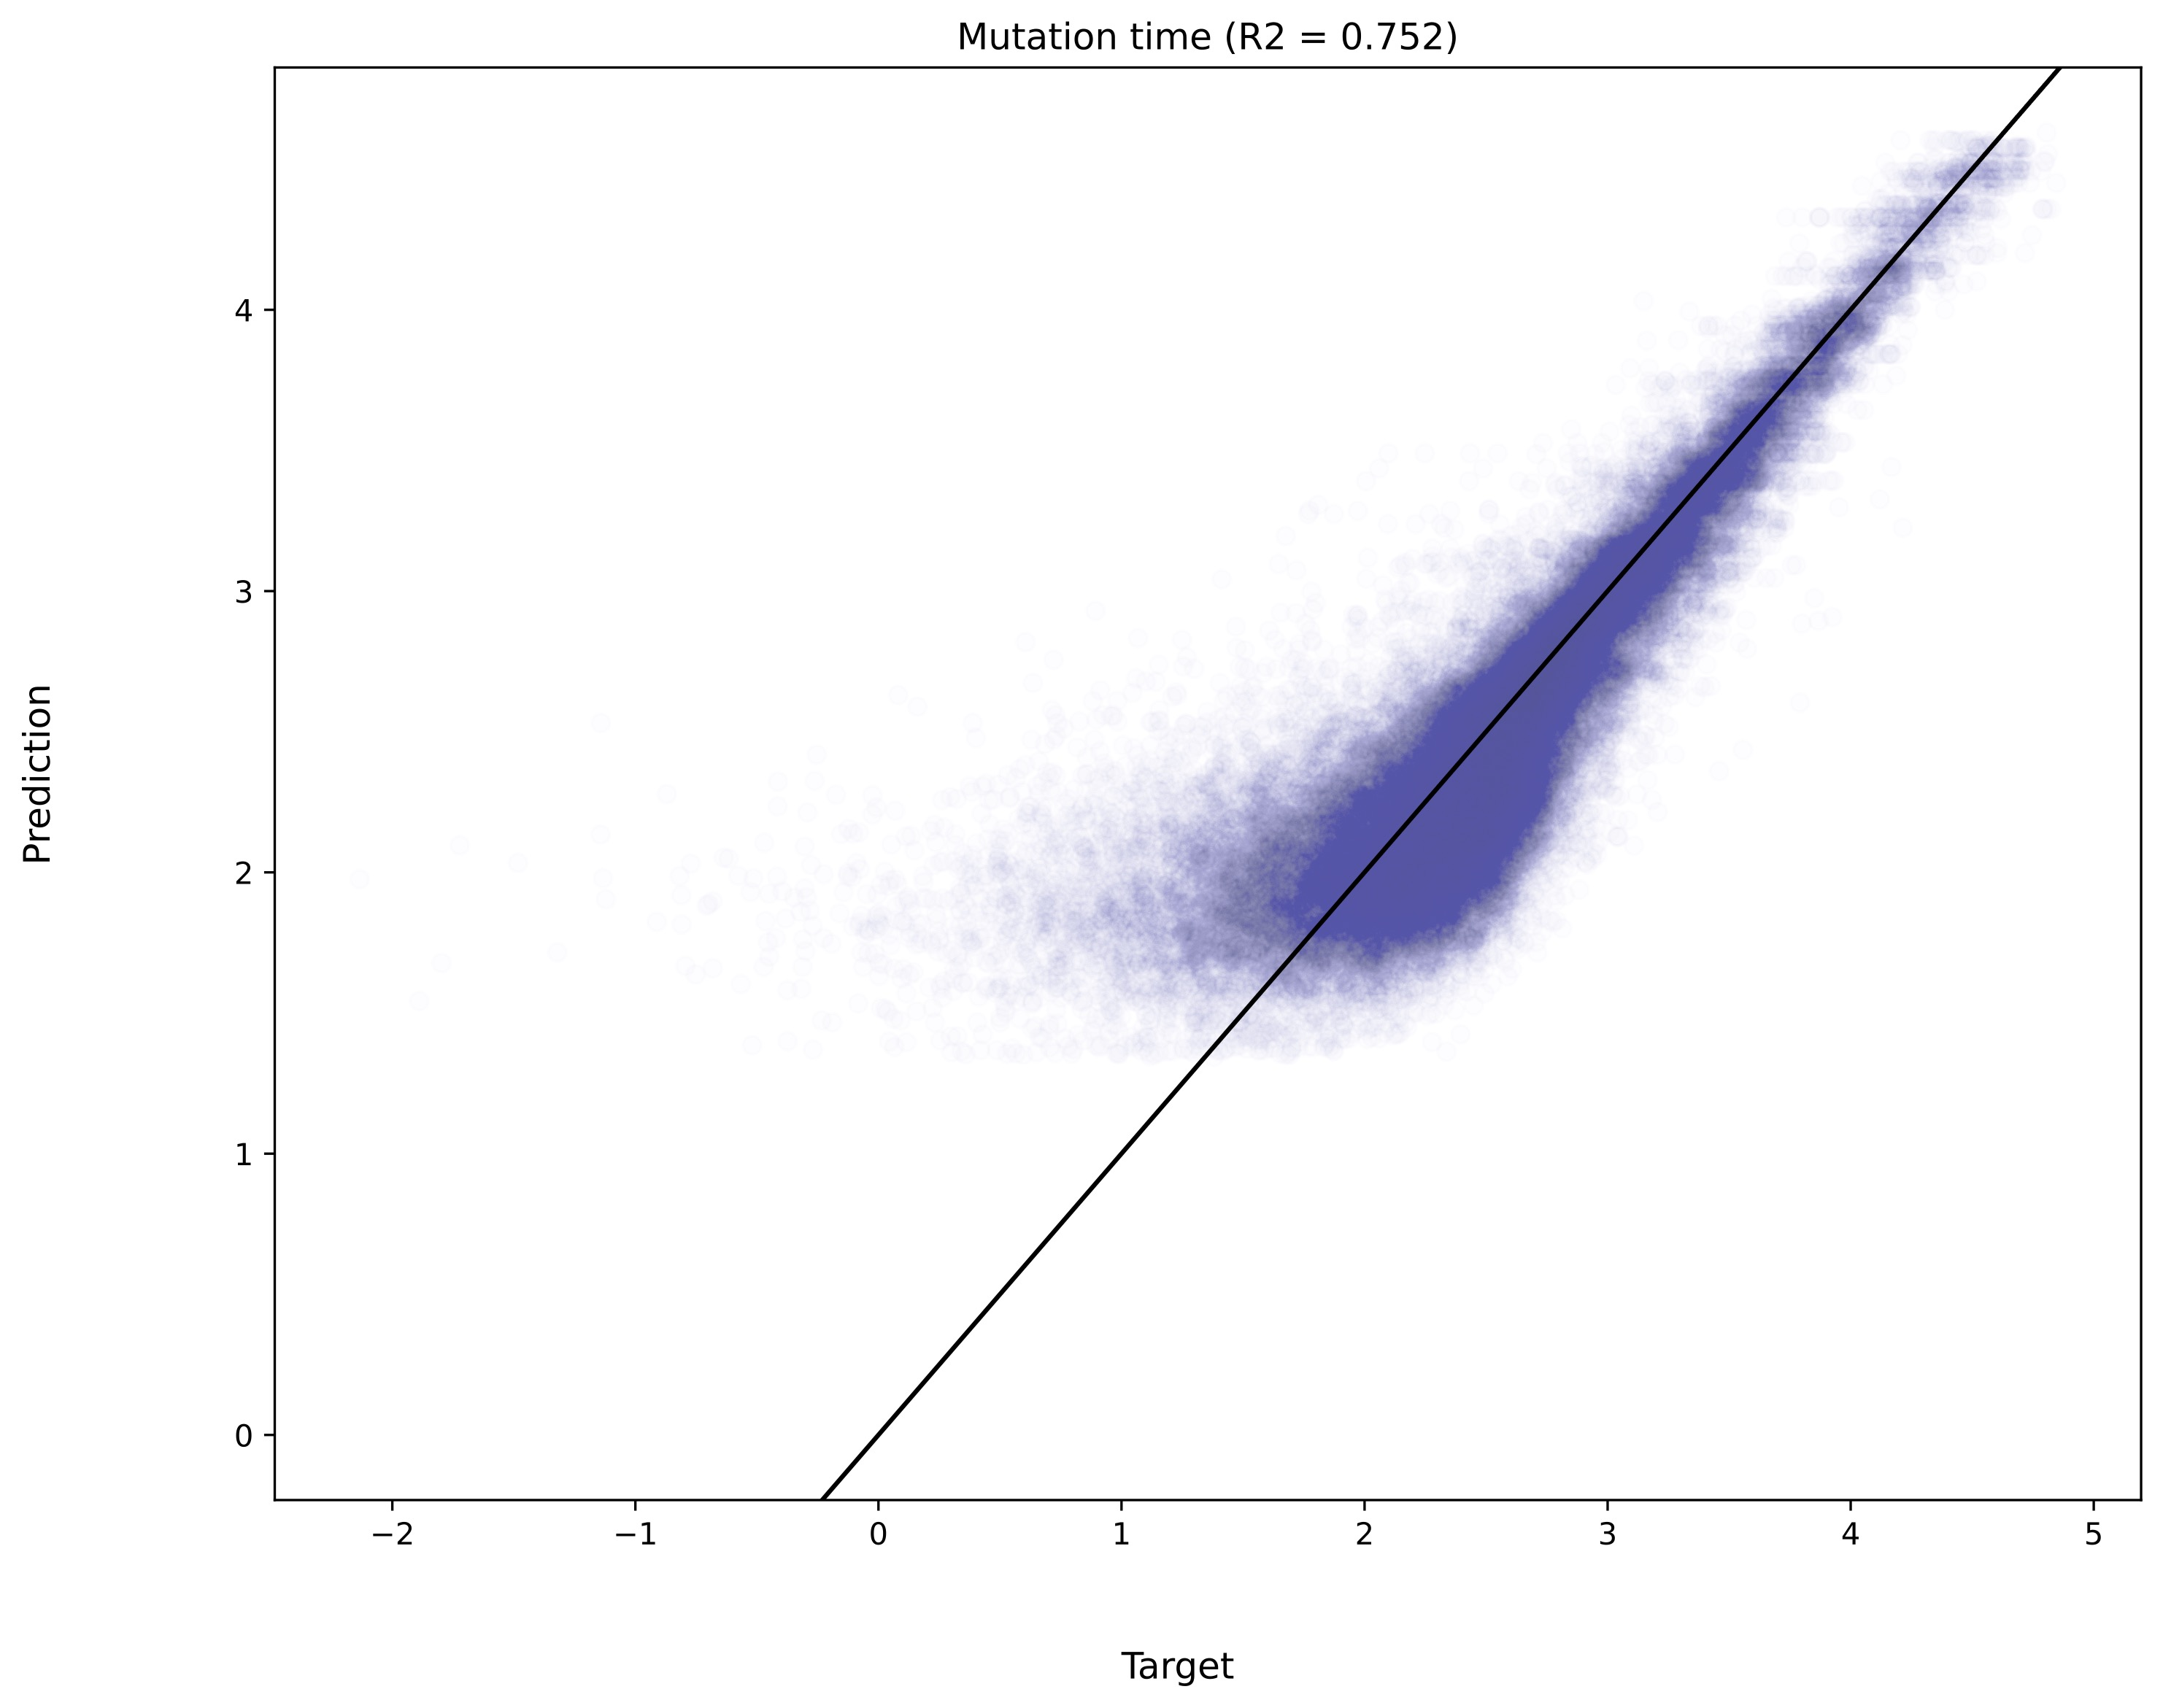
\includegraphics[width=\linewidth]{tsnn_figs/tsnn_ntrain_900_clen_10kb_mut-rate_2e-7_ssize_100_scatter_val.jpg}
    \caption{10Kb with mutation rate of $2\times10^{-7}$}\label{fig:10kb_7}
\end{subfigure}
\hfill
\begin{subfigure}[b]{.51\linewidth}
    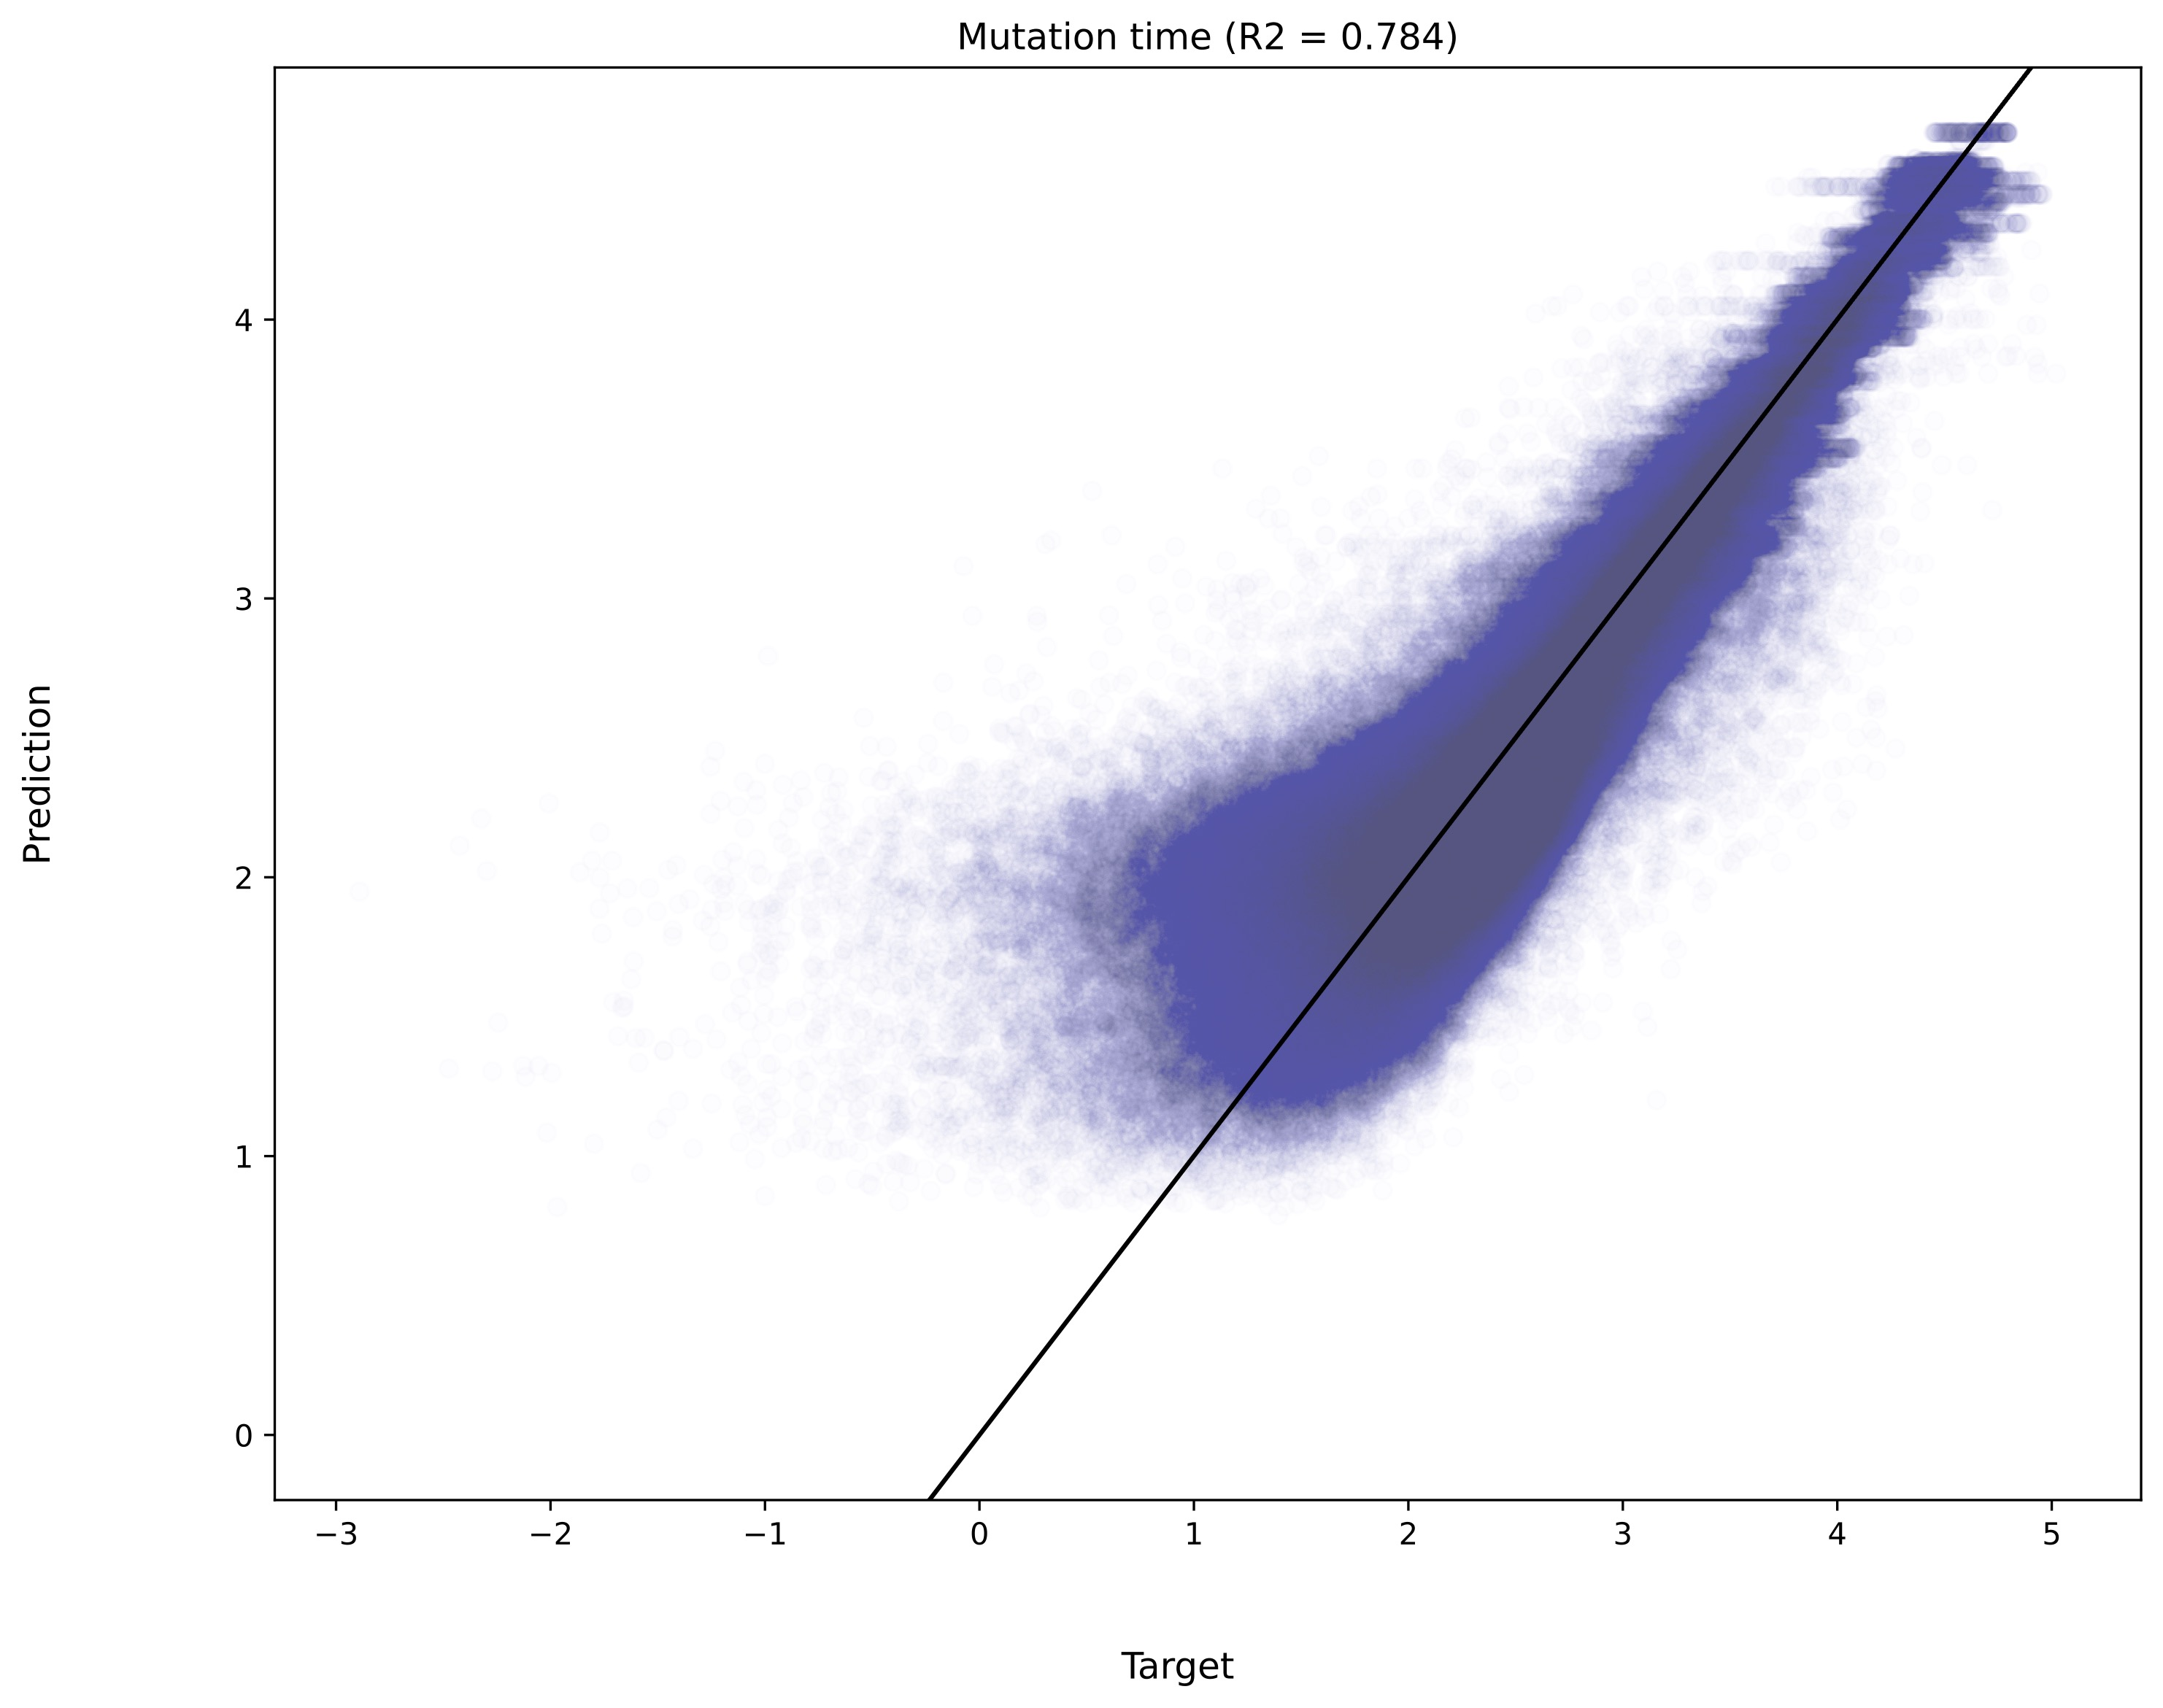
\includegraphics[width=\linewidth]{tsnn_figs/tsnn_ntrain_900_clen_10kb_mut-rate_2e-6_ssize_100_scatter_val.jpg}
\caption{10Kb with mutation rate of $2\times10^{-6}$}\label{fig:10kb_6}
\end{subfigure}
\hfill
\begin{subfigure}[b]{.51\linewidth}
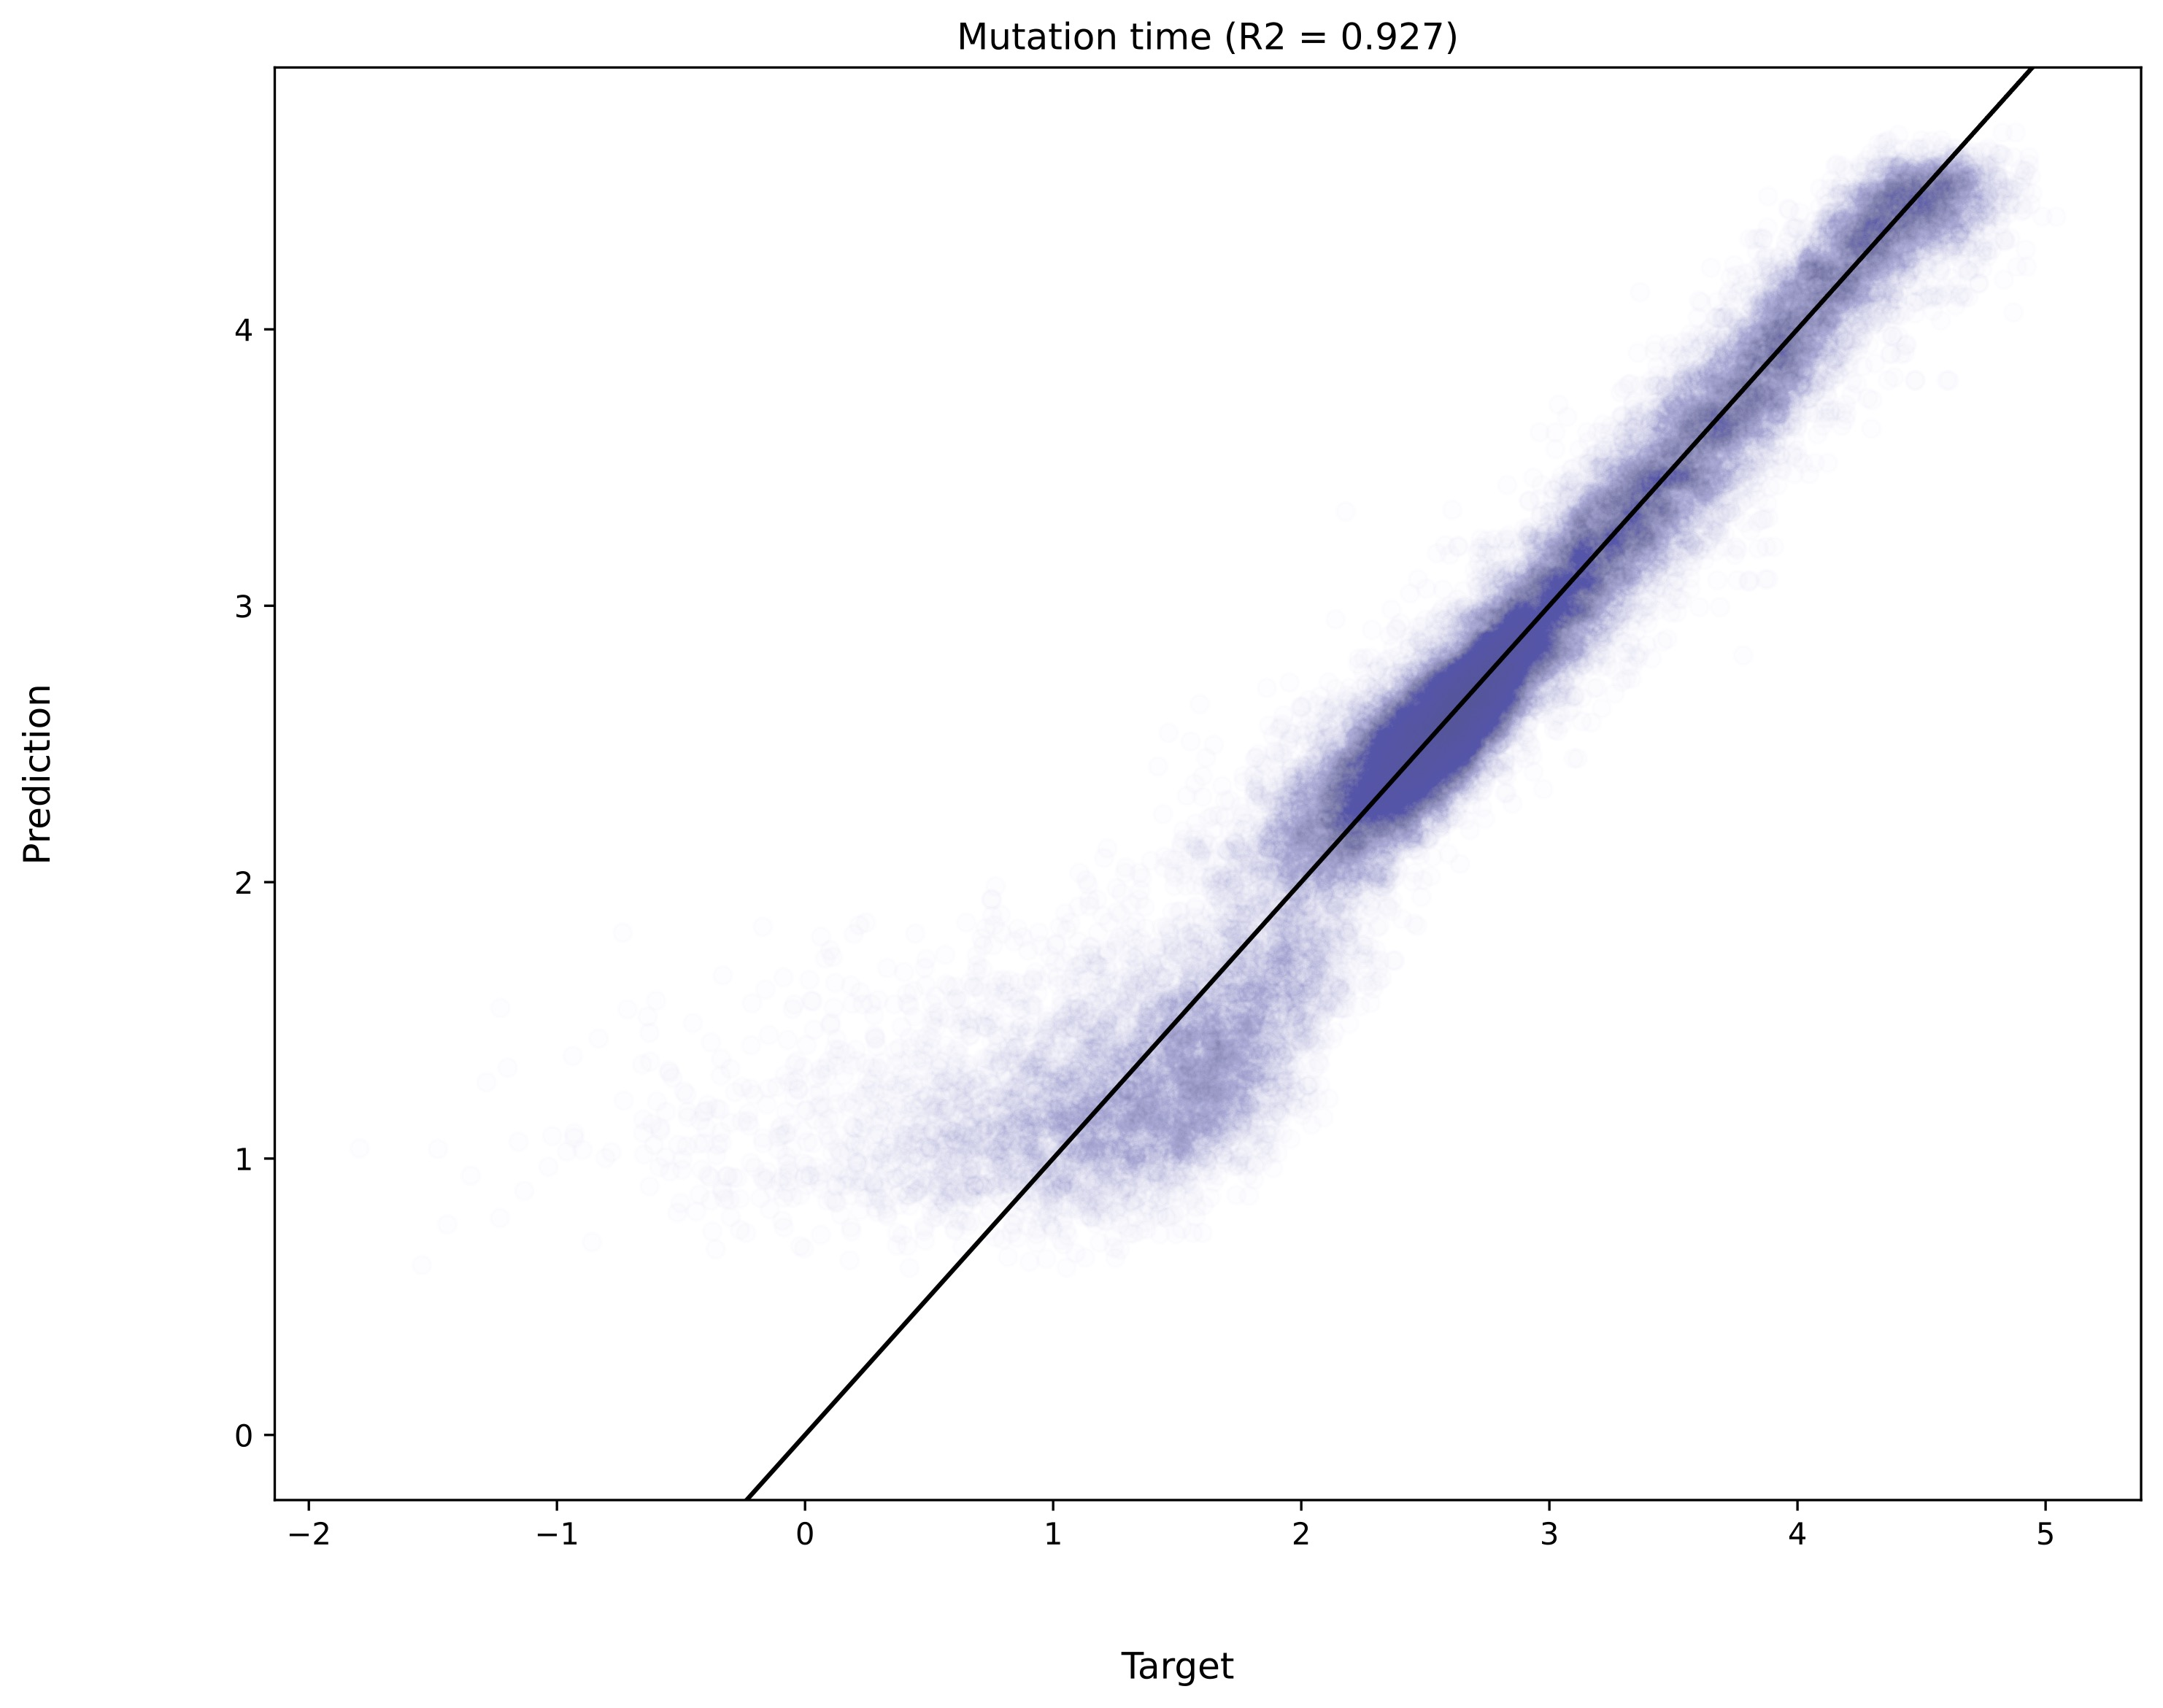
\includegraphics[width=\linewidth]{tsnn_figs/tsnn_ntrain_900_clen_1mb_mut-rate_2e-8_ssize_100_scatter_val_redone.jpg}
\caption{1Mb with mutation rate of $2\times10^{-8}$}\label{fig:1mb_8}
\end{subfigure}
\caption[The effect of number of mutations and chromosome length on accuracy]{
The effect of number of mutations and chromosome length on accuracy.
Scatterplots show predicted against target mutation times for 100 tree sequences.
Times are $\log_{10}$ transformed.
}
\label{fig:tsnn_vs_gnn}
\end{figure}


\section{Discussion}

Ancestral Recombination Graphs (ARGs) can solve many issues currently plaguing evolutionary inference, 
because it fully encodes evolutionary outcomes in a compact manner.
Treating the ARG as a latent parameter to be averaged out is not easy, because the state space is overwhelmingly large \citep{griffiths_ancestral_1996,nielsen_estimation_2000}.
More tractable approximations, such as the Sequentially Markovian coalescent (SMC), have been widely applied in evolutionary inference \citep{mcvean_approximating_2005, schraiber_methods_2015}, 
but the simplifying assumptions of these models limit their utility.
An alternative lies in shifting towards inferring a single plausible ARG \citep{kelleher_inferring_2019, speidel_method_2019, wong_general_2023}.
There is a clear need for methods that leverage an inferred ARG for population genetic inference
and to quantify potential gains in accuracy.
Nevertheless, it is not obvious how to use the all the information encoded in ARGs for inference,
and current studies either compute summary statistics based on ARGs or assume independency between marginal trees \citep{fan_likelihood-based_2023, hejase_deep-learning_2022}.


Our main goal has been to develop a framework that can leverage most of the information encoded in ARGs for evolutionary inference.
We show that our neural network, tsNN, can learn how to date mutations in an ARG,
outperforming likelihood-based models (tsNN $R^2=0.927$, tsdate $R^2=0.902$) \citep{wohns_unified_2022}.
By comparing performance on different training sets,
we demonstrate that the neural network learns to leverage both the mutation and recombination clocks to produce accurate estimates of mutation times.

% Problem of true vs inferred ARGs and errors
Although ARGs carry sufficient information for inferring evolutionary events,
ARG inference methods could significantly impact downstream applications.
Indeed, the two most widely adopted ARG inference programs, tsinfer and Relate, tend to overestimate small coalescence times and underestimate large ones \citep{y_c_brandt_evaluation_2022}.
In our mutation time inference task, we used the true ARGs for training and validation,
but some of these biases can be alleviated in a supervised machine learning framework by training on inferred ARGs, as opposed to true ARGs.

% Model mispecification
A trickier issue might arise when the true generative process, which yielded the real data, does not match that of the training data.
In our tests, we assumed that the training and validation data came from the exact model.
In the future, tests where we slightly alter the simulation model for training will aid in understanding the robustness of tsNN to model mis-specification.
Previous studies have shown that machine learning methods can be as robust to model mis-specification as their likelihood-based counterparts \citep{hejase_deep-learning_2022}.
A new approach to deal with the mis-specification issue, called Domain-Adaptive Networks, can mitigate mis-speficication by leveraging target-domain data in an unsupervised manner \citep{mo_domain-adaptive_2023}.

% Tasks at different levels
An exciting avenue for future research lies in expanding the tasks that tsNN can perform, 
what can be accomplished by developing different decoders.
For example, the rich information contained in the ARG could be used to distinguish between complex demographic models that are unidentifiable with allele frequency data (\eg the site frequency spectrum) \citep{schraiber_methods_2015, fan_likelihood-based_2023}.
The inference of selective sweeps has much to gain from leveraging ARGs,
mostly because it allows us to bypass the specification of a window size.
The span of ancestral haplotypes and edges naturally encode both the spatial and temporal scales over which processes impact variation,
and an ARG-based method can implicitly leverage this information.

% Conclusion
With the recent advances in scalable ARG inference methods, 
ARG-based evolutionary inference methods are still in its infancy.
A powerful framework that is able to efficiently leverage all the rich information contained in ARGs is needed.
The field of graph neural networks is ripe with ideas that can be applied to ARGs.
Indeed, we demonstrate that our method, tsNN, represents an important step in this direction,
but there still much work to be done in applying deep learning to gain new insights into past evolutionary events.
